%************************************************
\chapter{Hidden Markov Random fields for biological data clustering}\label{ch:HMRF} 
%************************************************
This chapter gives a theoretical overview of a Hidden Markov Random Field based approach aimed to be applied to cluster single cell in-situ hybridization gene expression data ``cubes" as described in chapter \ref{ch:singlecell} into $K$ clusters ($K \in [2,\infty[$). Subsequently, we will describe our approach for estimating $K$.

\section{Markov random fields}

	\subsection{Neighbourhood systems}\label{sec:neighbours}
Let $S$ be a finite set of sites, each of which represents one ``cube" of data. Given the 3D coordinates of each site, the first challenge to be able to use the spatial characteristics of the data in the clustering scheme will be to express the data and their spatial relationship in mathematically formal manner. To that end, stating from the spatial coordinates in 3D of each ``cube", instead of a list of isolated measurements, it is possible to build a connecting graph representing the same data and the spatial dependence between the `cubes". In the case of this study, each node of the graph will represent a ``cube" in the singe cell expression data. Nodes that are linked together by an edge will be spatially dependent upon each other.\\

With prior biological data, one can manually create the spatial dependency graph by linking nodes together that are known to be functionality similar. In the case of this study however, no such prior knowledge being available, it is necessary to define the spatial dependences in a different way.\\

The central hypothesis while developing this method is to assume that ``cubes" that are close to one another are more likely to belong to the same cell type (i.e cluster), the spatial dependencies connecting graph will then consist in a \emph{neighbouring graph} where  ``cubes" close to each other will be joined be edges.\\

As shown on figure \ref{fig:graph}, it was decided to use a first order neighbouring graph called $G$, i.e the 6 closest sites, to represent $S$.  using a first order neighbourhood system, i.e the 6 closest sites.\\

	\begin{figure}[h]
\centerline{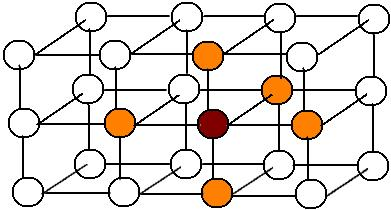
\includegraphics[width=0.5\linewidth]{gfx/chapter4/graph.jpg}}
\caption{{\bf First order neighbouring system.} In the chosen first order neighbouring system, each node in the graph (representing a ``cube" $\approx$ cell in the data) is linked to a maximum of 6 other cubes. The Markov property on the graph implies that the state of any node (the red one for example) can be fully determined by knowing the state of its neighbours (the orange ones).}\label{fig:graph}
	\end{figure}

In $G$, a \emph{clique} $C_1$ is a subset of nodes that are all interconnected, i.e it is possible to go from any the nodes in $C_1$ to any other node in $C_1$ by simply following one single edge. Let $C$ be the set of cliques of $G$. Because we chose a first order neighbouring system, $C$ is therefore the set of all the couple of sites that are neighbours of one another.

	\subsection{Gibbsian prior distribution}
Let a Random Field $Z$ be defined as a set of random variables $Z = \{Z_i , \forall i \in S\}$ where $Z_i \in [1,K]$. For every site $i \in S$, let $N(i)$ represent the set of its neighbours (see \ref{sec:neighbours}) and $\boldsymbol{z_{S-\{i\}}}$ a realization of the field restricted to $S-\{i\} = \{j \in S, j \neq i\}$. $Z$ is a \emph{Markov Random Field} if and only if it follows the Markov property at every site :

\begin{align}
\label{eq:markov1}
\forall i \in S, P_G (z_i \mid z_{S-\{i\}}) = P_G (z_i \mid z_j , j \in N(i))
\end{align}

Equation (\ref{eq:markov1}) states that the realization of the field, $z_{i}$ at any site $i \in S$ can be fully determined using only the state of its neighbours $N(i)$. In other words the probability that a ``cube" is in a given state depends only upon the state of its neighbours.\\
The Hammersley-Clifford theorem state that if $Z$ is a Markov Random Field, the joint distribution of the field $P_G$ follows a Gibbs distribution so that :

\begin{align}
\label{eq:prior}
P_G (\boldsymbol{z;\beta}) &= W(\boldsymbol{\beta})^{-1} \exp{(-H(\boldsymbol{z;\beta}))} \nonumber\\
&= \frac{e^{-H(\boldsymbol{z;\beta})}}{\sum\limits_{\boldsymbol{z'}} e^{-H(\boldsymbol{z;\beta})}}
\end{align}

with $H(\boldsymbol{z})$ the Energy function summed over the cliques $C$ of the graph $G$. Since we are working with a first order neighbouring system, $C$ is the set of all pairs of sites $(i,j)$ that are neighbours. We chose to consider $H$ as a function of vector $\boldsymbol{\beta} = (\beta_1, \hdots, \beta_K)$ containing $K$ parameters, one per cluster and $v_{i,j}$ a potential function set to 1 in our method. 

\begin{align}
\label{eq:Energy}
H(\boldsymbol{z}) = - \sum\limits_{i \in S}\beta_{z_i}\sum_{\substack{i,j\\neighbours}}v_{i,j}\times\boldsymbol{1}_{[z_i = z_j]} 
\end{align}

The denominator in (\ref{eq:prior}) where $\boldsymbol{z'}$ represents all the possible realizations of the field is a normalizing constant referred to as $W(\boldsymbol{\beta})$.\\

	\subsection{Single and multiple beta models in a biological context}
This model is closely related to a K-colour Potts model \cite{Wu82}. However, the unusual nature of the data used in this thesis lead to the idea of extending the model used mainly in the field of image segmentation. Indeed, the K-colour Potts model defines only one general spatial coherency parameter $\beta$ \cite{subudhi14,zhang14}. Importantly, the method presented here was extended by assigning one $\beta$ per cluster so that:
\begin{equation*}
\label{eq:beta}
\boldsymbol{\beta} = \operatorname{diag}(\beta_{1},...,\beta_{K})
\end{equation*}

 Interestingly, equation (\ref{eq:Energy}) is a decreasing function of every component of $\boldsymbol{\beta}$ and of the number of neighbouring ``cubes" in the field having the same class. This Energy function thus favours spatially regular partitions and a higher value of $\beta_h$, with $1 \leq h \leq K $ will amplify the smoothing effect, or coherence over cluster $h$.\\
 
 The reason why the model was extended to a multiple $\boldsymbol{\beta}$ parameter model, is inherent to the data used in this thesis. The first motivation is purely cytological. Indeed, in a biological context, it is expected that some tissues will be more spatially coherent than others. As mentioned in \ref{ch:background} and visualized in figure \ref{fig:cells}, tissues composed of different cell types may be interacting differently with their neighbours. For example, differentiated neural cells with long axons are likely to be in contact with numerous other cell types they go through leading to a low value for $\beta$. The second motivation for the extended model finds its root in the cell model described in \ref{sec:single_cell_insitu}. Indeed, the single cell nature the in-situ dataset is flawed by the inaccuracy of the cell model and as visualized in figure \ref{fig:cubeserrors} some ``cubes" may have inconsistent gene expression patterns. This will be especially true for cell types where cells are big.\\
 
 \subsection{Summary of the prior distribution parameters}

From this prior distribution are defined $K$ unknown parameters $\boldsymbol{\beta} = \operatorname{diag}(\beta_{1},...,\beta_{K})$ to be estimated by the model. It is important to note at this point that $W(\boldsymbol{\beta})$ is summed over all possible realizations of the field $Z$, this is an exponentially complex sum as the cardinality of $S$ rises. Therefore the computation of the normalizing factor becomes intractable very quickly. To address this problem, we are going to need to make some approximations in order to compute this quantity (see Mean Field Approximations).\\

\section{The emission model}

We have described the prior distribution of a Markov Random Field representing our partition, we now need to describe the relationship between $Z$ and the data.

\subsection{Conditional independence in the observed data}
As $Z$ is unknown a priori and represents the partition, let $Y$ be a set of random variables representing the observations (the in-situ hybridization data). The model requires a conditional independence assumption with regard to the observations $Y$ given the partition $Z$ so that, with $f_{z_i}$ the density function relative to cluster $z_i, i \in S$ (the realization of the field at node $i$):

\begin{align}
p(\boldsymbol{y} \mid \boldsymbol{z} ; \Theta) &= \prod_{i \in S} p(y_i \mid z_i ; \Theta) \nonumber\\
\label{eq:independence}
&= \prod_{i \in S} f_{z_i} (y_i \mid z_i ; \Theta)
\end{align}

Equation \ref{eq:independence} defines one unknown parameter per cluster: $\Theta = (\boldsymbol{\theta_1},...,\boldsymbol{\theta_K})$. It is interesting to note that this part of the model is equivalent to an independent mixture model \cite{mclachlan04}. Indeed, hidden Markov models can be viewed as independent mixture models where $Z$ is a set of independent, identically distributed random variables, which happens when $\beta = 0$.\\

Given a particular cluster $h \in [1,K]$ and M the set of considered genes, gene expression for each gene $m \in M$ in each cluster is modelled a Bernoulli distribution with parameter $\theta_{h,m}$. This leads to one unknown Bernoulli parameter per gene per cluster so that :

\begin{align*}
\Theta &= (\boldsymbol{\theta_1},...,\boldsymbol{\theta_K})\\
&= \left( \begin{array} {ccc}
\theta_{1,1} & \ldots  & \theta_{1,_K}\\
\vdots & \ddots & \vdots\\
\theta_{M,1} & \ldots & \theta_{M,_K} \end{array} \right)
\end{align*}

	\subsection{Full likelihood of the Hidden Markov random field model}

The conditional density function $f_i, i \in S$ can be expressed as :

\begin{align}
f_i(y_i \mid z_i ; \Theta) &= f_i(y_i \mid z_i ; \boldsymbol{\theta_{z_i}}) \nonumber\\ 
&= \prod_{m \in M} \theta_{z_i,m}^{y_{i,m}} \times (1-\theta_{z_i,m}^{1-y_{i,m}})
\end{align}

Looking at both fields $Z$ and $Y \mid Z$ together, the complete likelihood of the model is expressed as :

\begin{align}
\label{eq:likelihood}
P_G(\boldsymbol{y},\boldsymbol{z} \mid \Theta, \boldsymbol{\beta}) &= f(\boldsymbol{y} \mid \boldsymbol{z}, \Theta)P_G(\boldsymbol{z} \mid \boldsymbol{\beta})\nonumber\\
&= \frac{exp\{{-H(\boldsymbol{z} \mid \boldsymbol{\beta})} + \sum\limits_{i \in S}log f_i(y_i \mid z_i, \theta_zi)\}}{\sum\limits_{z'} e^{-H(\boldsymbol{z})}}
\end{align}

Because equation (\ref{eq:likelihood}) is a Gibbs distribution, using the Hammersley-Clifford theorem we can conclude that the conditional field $Y$ given $Z =\boldsymbol{z}$ is another a Markov Random Field with the Energy function 
\[H(\boldsymbol{z} \mid \boldsymbol{y}, \boldsymbol{\beta}, \Theta) = H(\boldsymbol{z} \mid \boldsymbol{\beta}) - \sum\limits_{i \in S} log f_i(y_i \mid z_i, \Theta)\]

In our case, the goal is to recover the unknown realization of $Z: \boldsymbol{z}$. To this end we need to maximize the values of all the parameters of the model $\boldsymbol{\psi} = (\boldsymbol{\Theta}, \boldsymbol{\beta})$. Additionally, choosing the unknown value $K$ will also be crucial (\todo{ref to chosing K}).

\section{Parameter estimation using the EM algorithm}
As mentioned before, the aim is to assign each cell $i$ to one of the $K$ possible clusters. To do so, it is interesting to consider the Maximum Posterior Marginal (MPM) that maximizes $P(Z_{i}=h|\boldsymbol{y}, \boldsymbol{\psi})$, where the $\boldsymbol{\psi}$ are unknown and need to be estimated.\\

The Expectation Maximisation \cite{dempster77} (EM) principle can be applied to this end. After initializing the clusters $\boldsymbol{z}$,  choosing $\boldsymbol{\psi}^{l+1}$ at iteration $(l+1)$ allows the maximization of the model's expectation $Q(\boldsymbol{\psi} \mid \boldsymbol{\psi}^{l})$ defined as:

\begin{align}
Q(\boldsymbol{\psi} \mid \boldsymbol{\psi}^{l}) &= \sum\limits_{\boldsymbol{z}} p(\boldsymbol{z} \mid \boldsymbol{y} ; \boldsymbol{\psi}^{l}) log\:p(\boldsymbol{y},\boldsymbol{z};\boldsymbol{\psi}) \nonumber\\ 
\label{eq:decomposed}
&= \underbrace{\sum\limits_{\boldsymbol{z}} p(\boldsymbol{z} \mid \boldsymbol{y} ; \boldsymbol{\psi}^{l}) log\:p(\boldsymbol{y} \mid \boldsymbol{z} ; \Theta)}_{R_y(\Theta\mid \boldsymbol{\psi}^l)} \nonumber\\
 &+ \underbrace{\sum\limits_{\boldsymbol{z}} p(\boldsymbol{z} \mid \boldsymbol{y} ; \boldsymbol{\psi}^{l}) log\:p(\boldsymbol{z} \mid \boldsymbol{\beta})}_{R_z(\boldsymbol{\beta}\mid \boldsymbol{\psi}^l)}
\end{align}

The decomposition in (\ref{eq:decomposed}) allows to consider separately the maximization of $R_y(\Theta\mid \boldsymbol{\psi}^l)$ and $R_z(\boldsymbol{\beta}\mid \boldsymbol{\psi}^l)$:


\begin{align*}
\Theta^{l+1} &= arg\:\underset{\Theta}{max}\:R_y(\Theta\mid \boldsymbol{\psi}^l)\\
\boldsymbol{\beta}^{l+1} &= arg\:\underset{\boldsymbol{\beta}}{max}\:R_z(\boldsymbol{\beta}\mid \boldsymbol{\psi}^l)
\end{align*}

$R_y$ can be estimated in the E step by using equation (\ref{eq:independence}) so that:

\begin{align*}
R_y(\Theta\mid \boldsymbol{\psi}^l) &= \sum\limits_{\boldsymbol{z}} p(\boldsymbol{z}\mid \boldsymbol{y} ; \boldsymbol{\psi}^{l})\;\sum\limits_{i \in S}\: log\: f_{z_i} (y_i ; \Theta)\\
&= \sum\limits_{i \in S} \sum\limits_{h=1}^{K}\; \left[log\: f_{h} (y_i  ; \Theta) \right] \; p(Z_i = h \mid \boldsymbol{y};\boldsymbol{\psi}^{l})
\end{align*}  

Therefore, at each iteration computing the following probably is required in the E step:

\begin{align*}
t_{i\,h}^{m+1} = p(Z_i = h \mid \boldsymbol{y};\boldsymbol{\psi}^{l})
\end{align*}

Computing this conditional probability is problematic because of the dependence between neighbouring ``cubes", and an exact value cannot be obtained without considerable computing resources. Indeed, each point being dependent upon its neighbours, and the neighbours being themselves dependent upon their neighbours, unsurprisingly computing these conditional probabilities becomes exponentially complex as the number of connected nodes in the graph grow. Additionally, as mentioned previously, the problem is the to compute the value of the normalizing constant $W(\boldsymbol{\beta})$.\\

To compute those quantities, approximations are needed. Methods to do so include Besag's pseudo-likelihood \cite{Besag75} to compute $W(\boldsymbol{\beta})$, and simulating the posterior distribution of $Z$ given $\boldsymbol{y}$ with the parameters at iteration $(l)$, with a Gibbs sampler to estimate $t_{i\,h}^{m+1}$ \cite{Chalmond89}.\\

However, another method exists, the mean field approximation originally proposed in the field of statistical mechanics. Since then, it has been used in a variety of fields including computer vision \cite{Yuille90} and more recently to approximate the distribution of both $W(\boldsymbol{\beta})$ (with a single $\beta$) and $t_{i\,h}^{m+1}$ \cite{Zhang92}. I present here the extension of this method to a model with one $\beta$ parameter per cluster.

\section{Mean field approximations}

The idea behind this approximation is to compute intractable quantities at any point $i \in S$ by setting all the other sites in the field to their mean values. Keeping in mind the Markov property expressed in equation (\ref{eq:markov1}), when considering a single site $i \in S$, setting all the other sites in the graph to a defined value is equivalentm, in the case of a MRF, to setting the values of $N(i)$ only.\\

When computing $t_{i\,h}^{m+1}$, the mean fields approximation yields the following fixed point equation for $i \in S$ and $1 \leq h \leq K$ \cite{Dang98}:

\begin{align}
\label{eq:fixedpoint}
t_{i\,h}^{m+1} \approx \frac{f_{h} (y_i;\boldsymbol{\theta}_{h}^m)\; exp\{\beta_h^m \: \sum_{j \in N(i)} t_{j\,h}^{m+1}\}}{\sum_{u=1}^K \: f_{u} (y_i;\boldsymbol{\theta}_{u}^m)\; exp\{\beta_u^m \: \sum_{j \in N(i)} t_{j\,u}^{m+1}\}}
\end{align}
\todo{write the fixed point algorithm}

For the normalizing constant $W(\boldsymbol{\beta})$, by applying the mean-field approximation, using equation (\ref{eq:Energy}), $W(\boldsymbol{\beta}$ can be written as:

\begin{align*}
W(\boldsymbol{\beta}) = \sum\limits_{\boldsymbol{z'}} exp(-H(\boldsymbol{z'})) \approx \sum\limits_{i \in S}\;\sum\limits_{\boldsymbol{z_i}} exp(-H(\boldsymbol{z_i})) = \sum\limits_{i \in S}\;\sum\limits_{\boldsymbol{z_i}} exp(\beta_{z_i}\sum\limits_{N(i)}[z_i=z_j])
\end{align*}

With this new set of equations, it becomes possible to estimate all quantities needed in the E step in order to compute the model's expectation.\\

\section{Maximization}
After the E step, maximizing $\boldsymbol{\psi}$ is relatively straightforward. For $\Theta$, once the the $t_{i\,h}^{m} = p(Z_i = h \mid \boldsymbol{y};\boldsymbol{\psi}^{l})$ have been computed during the E-step, those probabilities may be used to assign each cell to its most probable cluster at step $l$. Once the new partition is created, the values of $\Theta$ that maximize the model's expectation can be computed iteratively for cluster $h \in [1,K]$ and gene $m \in M$ with function $Expr_{h,m}$ the number of cells expressing gene $m$ in cluster $h$ and function $Num_h$ the total number of cells in cluster $h$.

\begin{align*}
\theta_{m,h}^{l+1} = arg\:\underset{\Theta}{max}\:R_y(\Theta\mid \boldsymbol{\psi}^l) = \frac{Expr_{h,m}}{Num_h}
\end{align*}

In order to maximize $\boldsymbol{\beta}^{l+1}$, an iterative approach such as the gradient ascent algorithm, the positive version of the gradient descent algorithm \cite{burges2005} can be used for each $\beta_h^{l+1}, h \in [1,K]$ over the function $R_z(\boldsymbol{\beta}\mid \boldsymbol{\psi}^l)$. \\
\todo{write the gradient ascent algorithm}


The described EM algorithm, summarized in \todo{write EM algo} leads, after convergence, to a partition over $K$ clusters that finds a local maximum of the model's expectation. Importantly, maximum reached is only a local one as indeed the EM algorithm does not guarantee to reach the global maximum of a function. It is interesting to note that this fact makes the initialization of the algorithm a crucial step as I will develop in \todo{link to init schemes}.\\

The partition computed is still over $K$ clusters, consequently, a method to choose the value $K$ is still needed.

\section{Estimating K}
Without any prior knowledge, choosing the right number of clusters $K$ is challenging. I decided to use an {\it{a posteriori}} method relying on the final log Likelihood of the model derived from equation (\ref{eq:likelihood}):

\begin{align*}
log\;L(\boldsymbol{\psi}) = 	log\;P_G(\boldsymbol{y},\boldsymbol{z} \mid \Theta, \boldsymbol{\beta})
\end{align*}

Because $Log\;L(\boldsymbol{\psi})$ monotonically increases with the number of parameters of the model, the BIC approach penalizes the addition of new parameters to the model. Let $P$ be the total number of parameters in the model and $N$ the cardinality of $S$, the BIC is expressed as:

\begin{align*}
\label{eq:BIC}
- 2\; log\:L(\boldsymbol{\psi}) + P\:log\:N
\end{align*}

By computing the final likelihood for a large range of possible $K$ values, the minimal resulting BIC will be chosen as the optimal number of classes, $\hat{K}$. When applied to the biological data however, this approach is not ideal as I will describe later in this thesis (see \todo{ref biological BIC}) but yields good results when applied to simulated data (see simulations \todo{ref next chapter}).\\

\section{Summary}
The goal was to allocate the $S=32,203$ ``cubes" described above in chapter \ref{ch:singlecell} into $K$ clusters, where $K$ is unknown, using the binarised matrix of $M=86$ gene expression measurements, $Y$. To incorporate spatial information into the clustering scheme, I assumed that $Z$, the (latent) vector of length $S$ that describes the allocation of cells to clusters, satisfies a first-order Markov Random Field (MRF), where the probability that a cell is allocated to a given state depends only upon the states of its immediate neighbours (Figure \ref{fig:neighbours}). Additionally, within cluster $h$ $(h \in [1,K])$, I assumed that the expression of gene $m$ follows a Bernoulli distribution with parameter $\theta_{m,h}$. The $M \times K$ matrix  $\Theta$ denoting the full set of Bernoulli parameters. In a typical MRF, the degree of spatial cohesion is determined by a single parameter $\beta$, which is assumed to be constant for all clusters \cite{subudhi14,zhang14}. However, in the context of tissue organisation, it is reasonable to expect that the degree of spatial cohesion will differ between clusters; consequently,  a separate value of $\beta$ is estimated for each of the $K$ clusters.\\

To estimate the parameters of the model an Expectation-Maximisation (EM) based approach has been used in conjunction with mean-field approximations to infer intractable values \cite{Celeux01}. Finally, to choose the optimal number of clusters, $K$, the use the Bayesian Information Criterion (BIC) has been proposed.\\

The next step is to validate the method's behaviour and to assess the quality of the results compared to the other non-spatial clustering schemes described in chapter \ref{ch:non_spatial_clustering_visualization}. Consequently, I decided to perform a simulation study that I will describe in the next chapter.

%*****************************************
%*****************************************
%*****************************************
%*****************************************
%*****************************************
